\documentclass[12pt]{article}
\usepackage{latexblog}

% ============================================================
% Blog Metadata
% ============================================================
\blogtitle{Android Develop:横屏布局}
\blogdate{2019-02-21}
\blogtags{Android, 移动端, 闲话编程}
\bloglang{zh}
\blogsummary{}

\begin{document}
\makeblogtitle

虽然我们可以将UI设计的尽可能的响应式，但是也可以为横屏应用单独进行布局达到更好的效果。横屏布局是通过layout-land文件夹中的同名layout文件实现的。

\section{创建landscape布局}\label{ux521bux5efalandscapeux5e03ux5c40}

在新版的Android Studio中，默认生产的工程中是没有layout-land文件夹的，我们也不必手动创建这样的文件夹。在design界面，可以快捷的创建横屏布局：

\begin{figure}
\centering
\pandocbounded{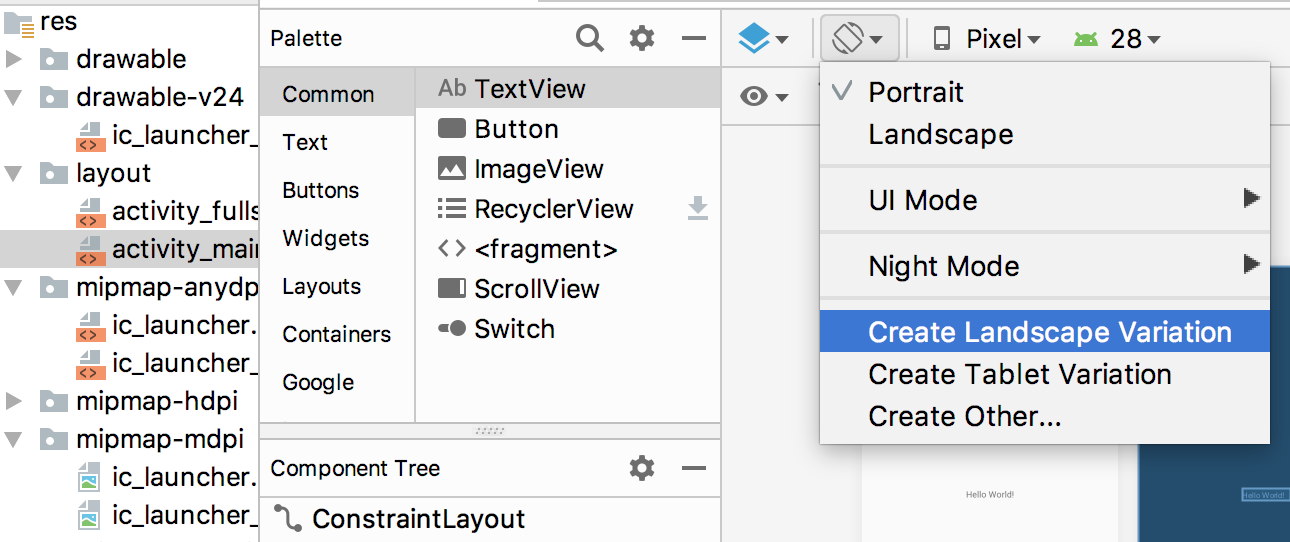
\includegraphics[keepaspectratio,alt={create land layout}]{images/create_land_layout.png}}
\caption{create land layout}
\end{figure}

\section{代码中的实现}\label{ux4ee3ux7801ux4e2dux7684ux5b9eux73b0}

值得注意的是，虽然land的布局文件已经加上了，但我发现我的界面在旋转的时候并没有生效（竖屏的时候旋转屏幕），还是显示的竖屏的设计界面，研究了一下发现问题所在：

\begin{Shaded}
\begin{Highlighting}[]
\NormalTok{\textless{}}\KeywordTok{activity}
            \OtherTok{android:name=}\StringTok{".SplashActivity"}
            \OtherTok{android:configChanges=}\StringTok{"orientation|keyboardHidden|screenSize"}
            \OtherTok{android:theme=}\StringTok{"@style/Theme.AppCompat.NoActionBar"}\NormalTok{\textgreater{}}
\end{Highlighting}
\end{Shaded}

可以看出android:configChanges中有orientation这一个mask，意味着当屏幕旋转时，安卓设备不会自己去处理这个事件，所以也就没有生效。解决方案有两种：

一个是删掉这个android:configChanges中的orientation选项，这样旋转屏幕的时候，android会销毁掉activity并重新创建一个，当然这时候如果有一些数据需要保存的话也就没有了。

另一个是保留这个选项，在代码中处理：

\begin{Shaded}
\begin{Highlighting}[]
\AttributeTok{@Override}
\KeywordTok{public} \DataTypeTok{void} \FunctionTok{onConfigurationChanged}\OperatorTok{(}\BuiltInTok{Configuration}\NormalTok{ newConfig}\OperatorTok{)} \OperatorTok{\{}
    \KeywordTok{super}\OperatorTok{.}\FunctionTok{onConfigurationChanged}\OperatorTok{(}\NormalTok{newConfig}\OperatorTok{);}

    \FunctionTok{setContentView}\OperatorTok{(}\NormalTok{R}\OperatorTok{.}\FunctionTok{layout}\OperatorTok{.}\FunctionTok{activity\_splash}\OperatorTok{);}
\OperatorTok{\}}
\end{Highlighting}
\end{Shaded}

这样不会销毁这个activity。

\begin{figure}
\centering
\pandocbounded{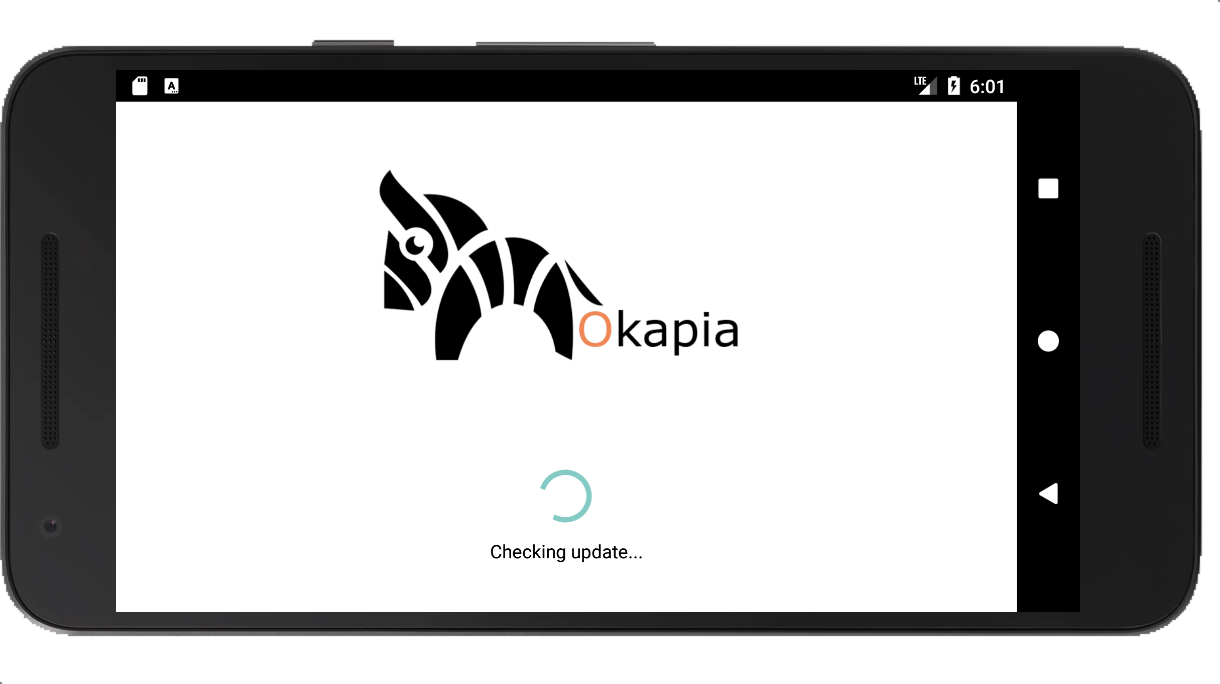
\includegraphics[keepaspectratio,alt={land layout}]{images/land_layout.png}}
\caption{land layout}
\end{figure}

\begin{figure}
\centering
\pandocbounded{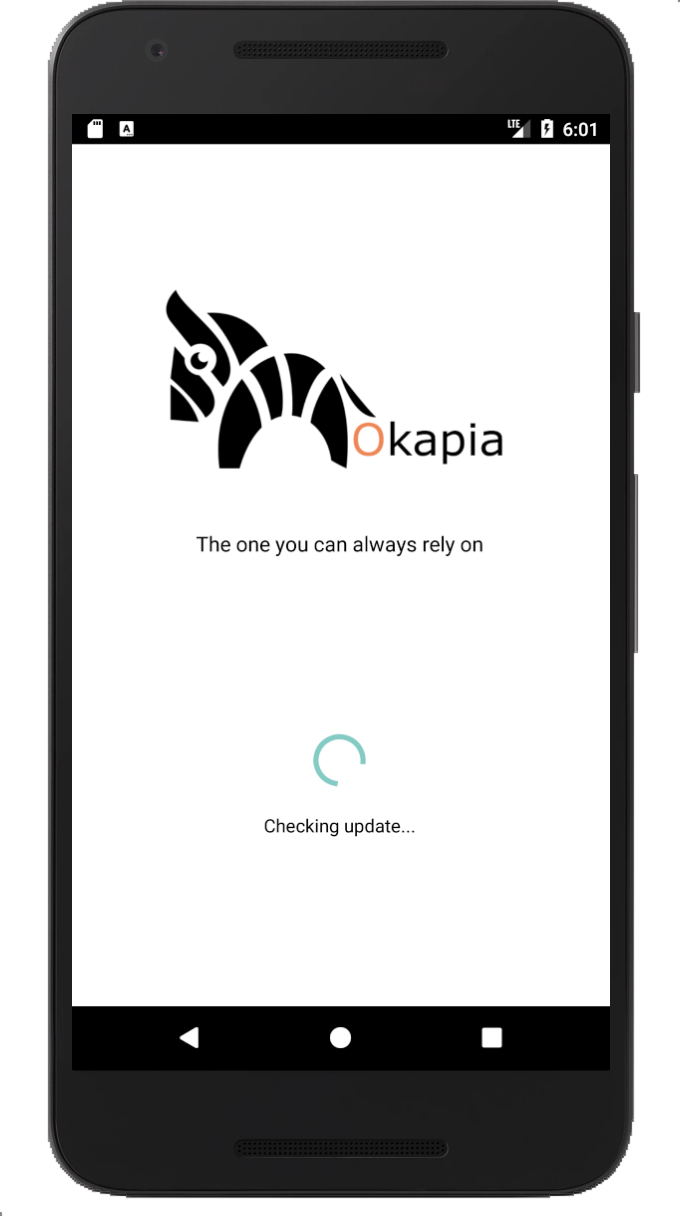
\includegraphics[keepaspectratio,alt={portrait layout}]{images/portrait_layout.png}}
\caption{portrait layout}
\end{figure}


\end{document}
